\documentclass[10pt,twocolumn,letterpaper]{article}
\usepackage[review]{cvpr}
\definecolor{cvprblue}{rgb}{0.21,0.49,0.74}
\usepackage[pagebackref,breaklinks,colorlinks,allcolors=cvprblue]{hyperref}
\usepackage{float}

\def\paperID{00000}
\def\confName{CVPR}
\def\confYear{2026}

\title{GlobalPuzzle: Jigsaw Puzzle Reassembly via Global Canvas Evaluation, Position Querying, and Genetic Search}
\author{Author Name\\Institution\\{\tt\small email@example.com}}

\begin{document}
\maketitle

\begin{abstract}
Jigsaw puzzle reassembly remains a highly challenging task, particularly when piece boundaries are irregularly eroded to simulate damage to cultural artifacts. On the GAP benchmark, existing methods achieve a perfect assembly accuracy of only 0.3\% on 5*5 puzzles, whereas humans can solve jigsaw puzzles with remarkably high accuracy. Humans typically approach puzzle solving by identifying potentially adjacent pieces, evaluating the current assembly, and iteratively performing complex operations such as adding pieces, replacing incorrectly placed pieces, and moving entire connected groups of pieces. However, existing methods face a fundamental limitation: approaches that leverage global visual information typically predict piece arrangements directly, making it difficult to explicitly perform such complex iterative operations, while search based methods can rearrange pieces but primarily rely on pairwise boundary compatibility, lacking global visual information to evaluate and guide the search process.

\noindent
To bridge this gap, we propose GlobalPuzzle, a jigsaw puzzle reassembly framework that integrates global canvas level evaluation, action guidance, and genetic search. By incorporating global visual information into the evaluation and optimization of candidate assemblies, GlobalPuzzle aims to resolve ambiguous adjacency relationships that are difficult to determine from irregularly eroded piece boundaries alone, enabling more flexible and globally informed puzzle reconstruction.
\end{abstract}

\section{Introduction}

Jigsaw puzzle reassembly with missing visual information is challenging due to the enormous search space and irregularly eroded piece boundaries.
An $N \times N$ puzzle has $(N^2)!$ possible arrangements, making the probability of randomly solving a $5 \times 5$ puzzle only $1/25! \approx 6.44695 \times 10^{-26}$.
Boundary erosion disrupts visual continuity, while smaller pieces provide less information for determining their positions and adjacency relationships.
Even advanced AI agents such as Claude Sonnet 5.5 Medium and Codex require approximately 10 minutes on average to solve a $3 \times 3$ GAP puzzle and rarely reconstruct $5 \times 5$ puzzles correctly.

\begin{figure}[H]
    \centering
    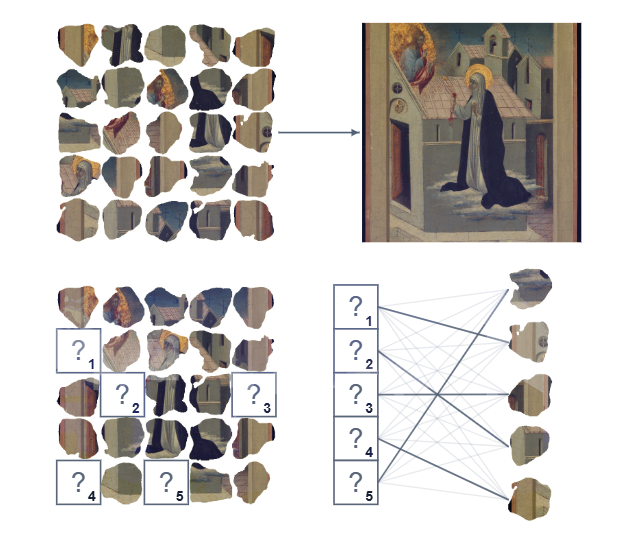
\includegraphics[width=\linewidth]{pic/Teaser.png}
    \caption{
       Fragment reconstruction: the top left shows irregular pieces in random order, the top right shows the complete image after placing the pieces correctly and using LAMA to fill in the gaps, and the bottom left shows the process in GlobalPuzzle of forming a position query for a current state and retrieving pieces.
    }
    \label{fig:agent_comparison}
\end{figure}

Existing methods face two major limitations. On the one hand, many deep learning approaches exchange information among fragments through attention mechanisms and directly predict or iteratively refine their arrangements. However, such feature interaction does not explicitly construct a spatially assembled image for visual evaluation. More importantly, these methods lack explicit mechanisms for preserving established fragment connections and moving connected groups as a whole. On the other hand, combinatorial optimization methods can explore different arrangements and preserve fragment relationships through genetic operations, but typically rely on pairwise boundary compatibility to evaluate candidate solutions. When fragment boundaries are severely eroded, local compatibility scores may be insufficient to determine whether an arrangement forms a globally coherent image.
When piece boundaries are severely damaged, the arrangement with the highest local compatibility score may not form a globally semantically coherent image.

Effective puzzle reassembly requires preserving reliable fragment connections while allowing connected groups to move and reorganize as a whole. Moving fragments independently may destroy correct local structures, while permanently fixing connected groups may preserve incorrect relationships and prevent further correction. Genetic algorithms provide a natural solution to this problem. Through crossover, shared fragment connections can be inherited and relocated as complete groups, while mutation and population diversity allow incorrect structures to be broken and recombined. However, effective search also requires reliable guidance for both fragment placement and candidate evaluation. Rather than relying solely on local boundary compatibility, these decisions should incorporate global visual information from the assembled image.

Motivated by these observations, we propose GlobalPuzzle, a jigsaw puzzle reassembly framework that integrates genetic search with global visual guidance. The genetic algorithm preserves and relocates shared fragment connections through crossover, while mutation and population evolution allow these structures to be continuously revised. Two neural networks guide offspring generation and candidate evaluation. The Global Evaluation Network takes a complete assembled canvas as input and predicts a continuous quality score between 0 and 1, serving as the fitness function for genetic search. The Position Query Network takes a partially assembled canvas as input, generates query tokens for unfilled positions, and interacts with all fragment features through a Transformer to predict suitable placements. By integrating structural inheritance, position based guidance, and global canvas evaluation, GlobalPuzzle enables flexible reconstruction while guiding the search using the visual coherence of complete candidate assemblies.

\section{Related Work}

\subsection{Direct Arrangement Prediction Methods}

Recent learning based approaches formulate jigsaw puzzle reassembly as an arrangement prediction or position estimation problem. JigsawGAN combines permutation classification with generative adversarial learning to exploit global image semantics for arrangement prediction. FCViT employs Vision Transformers to model relationships among fragments and directly regress their two dimensional coordinates. PuzLM converts fragments into discrete visual sequences and employs a sequence generation model to predict fragment positions autoregressively. DiffAssemble and JPDVT introduce diffusion models to iteratively recover fragment arrangements through pose denoising and positional encoding denoising, respectively. PuzzleFlow further combines Vision Transformers with discrete flow matching to iteratively predict and update fragment positions based on the current arrangement.

These methods leverage attention mechanisms to exchange visual information among fragments, allowing each fragment to incorporate information from other fragments. However, such global feature interaction does not necessarily construct a spatially assembled image. Even when positional information is incorporated, the model primarily operates on fragment representations rather than explicitly evaluating the visual coherence of a complete canvas. Furthermore, although some methods iteratively adjust fragment positions, they lack explicit mechanisms for identifying, preserving, and manipulating connected fragment groups. Consequently, complex reconstruction strategies, such as preserving established connections, replacing incorrectly positioned fragments, and moving connected groups as a whole, are not explicitly supported.

\subsection{Compatibility Based Search and Optimization}

Another line of research decomposes jigsaw puzzle reassembly into fragment compatibility estimation and combinatorial optimization. Traditional methods estimate pairwise compatibility using color differences, gradient continuity, and texture information, while learning based methods employ neural networks to predict adjacency compatibility between fragments. Given these compatibility scores, greedy algorithms progressively connect fragments with high compatibility, linear programming methods jointly optimize fragment positions under global constraints, and genetic algorithms explore candidate arrangements through selection, crossover, and mutation. Some genetic algorithms further preserve existing fragment connections during crossover, allowing connected groups to be rearranged as a whole.

Unlike direct prediction methods, search based approaches can explicitly explore different arrangements and perform more flexible structural operations. However, their objective functions primarily rely on local pairwise compatibility rather than the visual coherence of the complete assembled image. When fragment boundaries are severely eroded, local compatibility information may become insufficient to reliably distinguish candidate arrangements. Therefore, integrating global visual evaluation of complete canvases with explicit structural operations provides a promising direction for guiding the search and optimization of jigsaw puzzle reconstruction.

\begin{figure*}[!t]
    \centering
    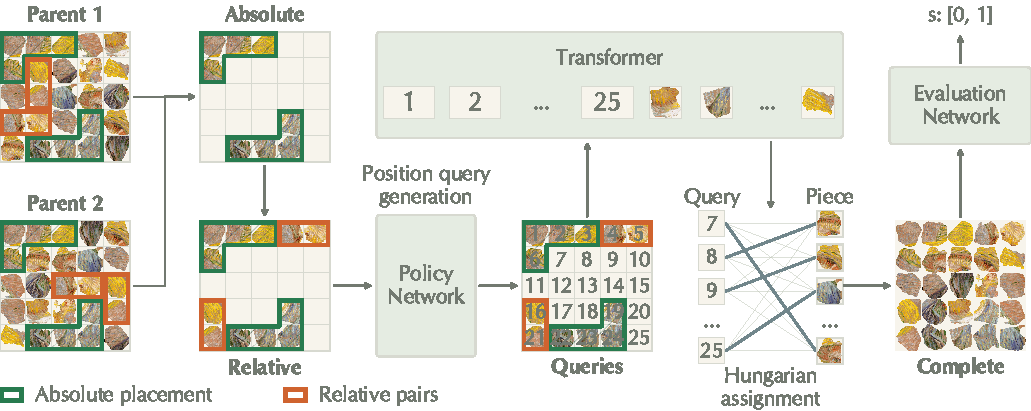
\includegraphics[width=\textwidth]{pic/all.pdf}
    \caption{
       Core architecture: offspring inherit the connectivity from parent samples, then use a neural network to generate position queries to fill fragments, which are then scored by an evaluation network.
    }
    \label{fig:all}
\end{figure*}

Although these methods can explore different puzzle configurations through combinatorial optimization, their objective functions are primarily based on local pairwise compatibility rather than the visual coherence of the complete assembled image. In contrast, GlobalPuzzle integrates learned global canvas evaluation with genetic search. It generates candidate arrangements through position based queries, preserves piece relationships through structural inheritance, and evaluates each assembled canvas using a visual fitness network. The resulting global fitness scores guide the search and optimization process.


\section{Method}

\section{Experiments}

\section{Conclusion}

{\small
\bibliographystyle{ieeenat_fullname}
\bibliography{references}
}

\end{document}
